\section{Diagramm mit GraphML}
\prc

\subsection{Aufbau der GraphML-Datei}

Die Elemente innerhalb der GraphML-Datei sind in der selben Reihenfolge wie sie in der XERML-Datei des Benutzers stehen. Bei unseren Testmodellen sind zuerst die Entitytypen und hinterher die Beziehungstypen gelistet. Aus diesem Grund sind in der GraphML-Datei zuerst die Entitytypen und Beziehungstypen als \textit{node}-Elemente. Zwischen den Elementen die die Beziehungstypen repräsentieren sind die \textit{edge}-Elemente enthalten um die Knoten miteinander zu verbinden.

\subsection{Beispiel eines ER-Diagramms in yEd}

In der nachfolgenden Abbildung \ref{yedERD} sieht man ein Beispiel für ein ER-Diagramm in yEd. Das Diagramm wurde vollständig durch das Tool erzeugt. Einzig die endgültige Anordnung der Elemente wurde durch die Layout-Algorithmen von yEd übernommen.

\begin{figure}[!h]
	\begin{center}
		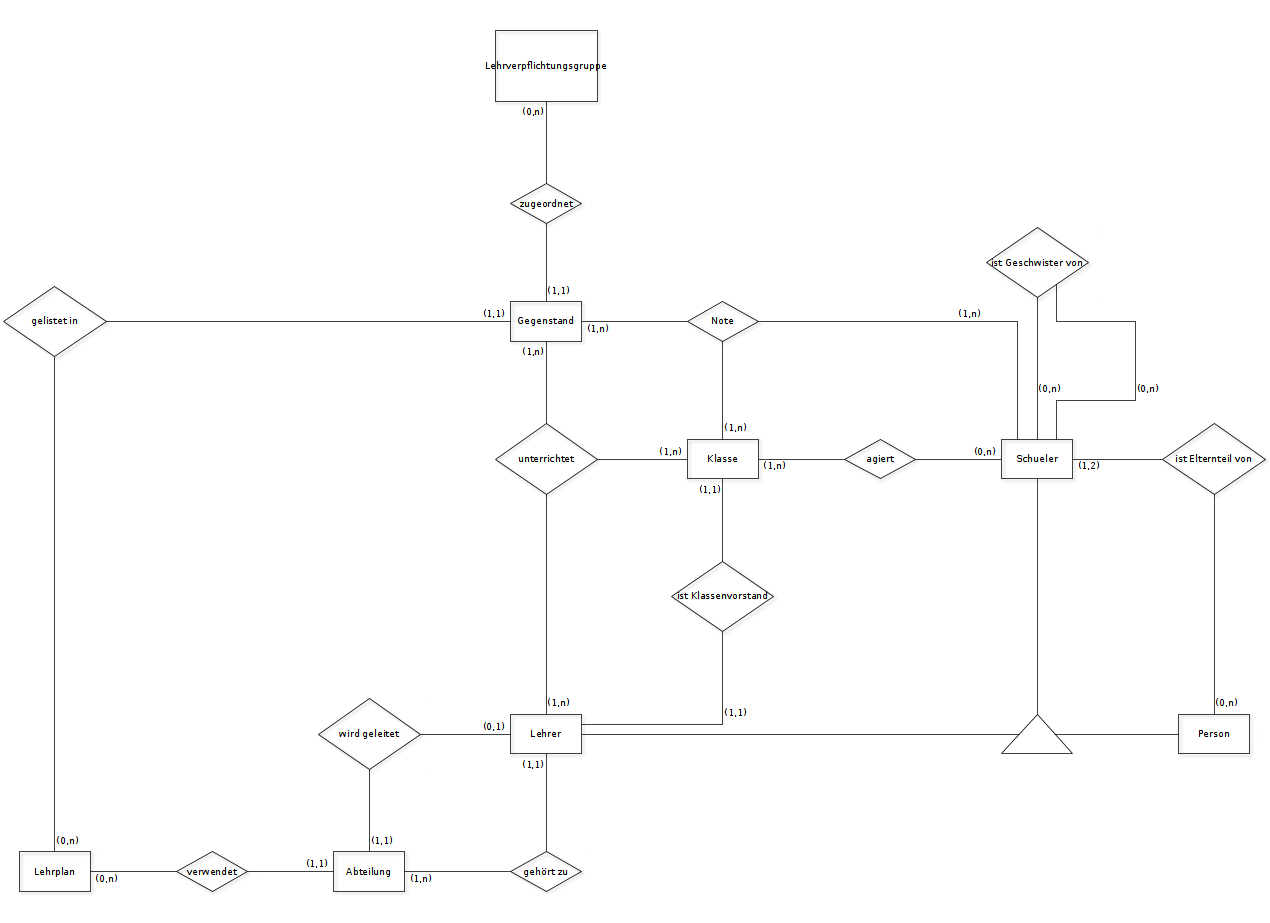
\includegraphics[width=11cm]{images/yedERD.png}
		\caption{ER-Diagramm des Datenmodells Schulinformationssystem}
		\label{yedERD}
	\end{center}
\end{figure}